\documentclass[11pt,pdftex,letterpaper]{article}
\usepackage[
    hdivide={1in,*,1in},
    vdivide={1in,*,1in},
]{geometry}

\usepackage{graphicx}
\usepackage{fancyhdr}
\pagestyle{fancy}
\usepackage{listings}
\usepackage{lastpage}

\setlength{\topmargin}{-.5in}
\setlength{\textheight}{9in}
\setlength{\oddsidemargin}{.125in}
\setlength{\textwidth}{6.25in}
\setlength{\headheight}{14pt}

\rhead{\thepage\ of \pageref{LastPage}}
\cfoot{\small{Boys Town National Research Hospital - Technology Core}}

\begin{document}
\vspace*{30ex}
\begin{center}
\textbf{Audiovisual Coordinate Response Measure Test}\\
\vspace{4ex}
Seth Bashford
\end{center}
\pagebreak
\tableofcontents
\pagebreak

\section{Goals}
\begin{itemize}
\item Develop a macOS application for design and administration of a coordinate response measure test
\end{itemize}

\section{Description}
This project provides a macOS application for running an audio-visual coordinate response measure test. The experimenter selects a number of testing parameters prior to starting the test as shown in Figure~\ref{fig:test-setup-window}.
\begin{figure}
\centering
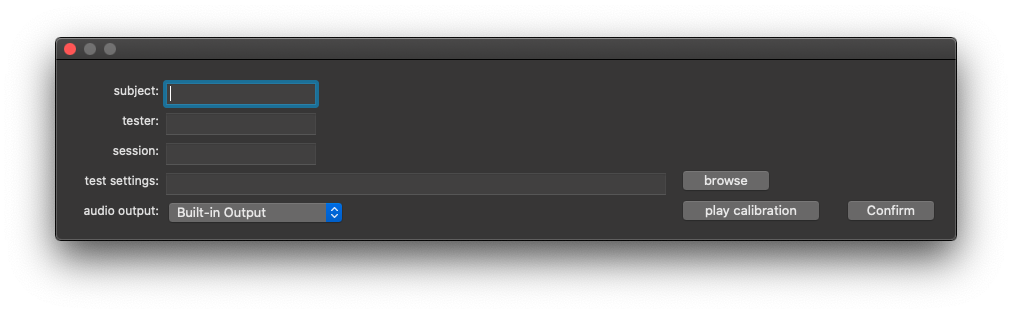
\includegraphics[width = 0.9\linewidth]{test-setup-window.png}
\caption{test setup window}
\label{fig:test-setup-window}
\end{figure}

The subject initiates each trial by pressing a button on a window located on the secondary screen/monitor. Figure~\ref{fig:subject-ready-window} shows the screen the subject sees before beginning a trial.
\begin{figure}
\centering

\includegraphics[width = 0.9\linewidth]{subject-ready-window.png}
\caption{subject window before trial}
\label{fig:subject-ready-window}
\end{figure}
Each trial begins with the playback of a random section of a masker where the masker is an audio file chosen by the tester prior to the start of the test. The masker fades in for 0.5 seconds to a level specified by the tester. After the masker finishes fading in a randomly selected target stimulus is played in conjunction with the masker where the target is chosen among a collection of audio files contained in a directory specified by the tester. Figure~\ref{fig:target-stimulus} shows such an example target stimulus.
\begin{figure}
\centering
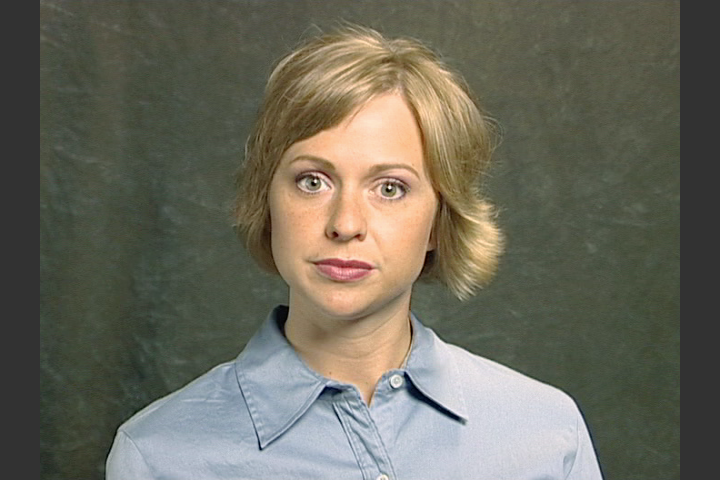
\includegraphics[width = 0.9\linewidth]{target-stimulus.png}
\caption{target stimulus}
\label{fig:target-stimulus}
\end{figure}
The target files are filtered to those having extensions of \textit{.mov}, \textit{.avi} or \textit{.wav}. If the tester specifies an “auditory-only” condition the target video is not shown. The target is played at a level dictated by an adaptive tracking rule of 1-up, 1-down for 2 reversals at a step size of 4 dB followed by 6 reversals at a step size of 2 dB. The initial target level is specified by the tester. A level of 119 dB SPL corresponds to a signal having a rms equivalent to that of a full-scale square wave. The targets are chosen with delayed replacement so that no two consecutive targets are the same. After the target finishes playing the masker fades out for 0.5 seconds. Once the masker has finished fading out the subject window is populated with 4 rows of 8 colored-number buttons whose colors are green, red, blue and white as shown in Figure~\ref{fig:subject-response-window}. 
\begin{figure}
\centering
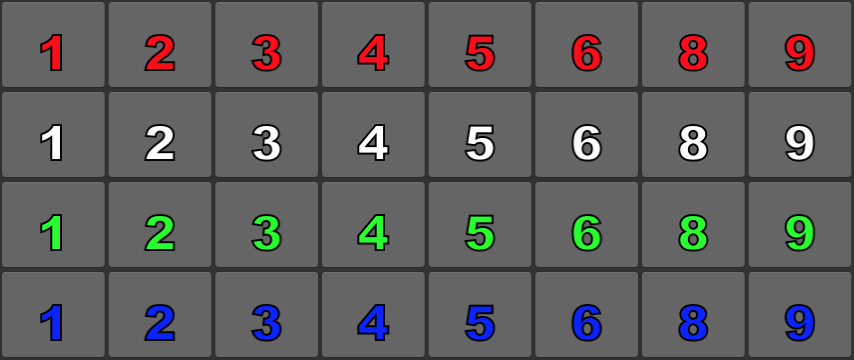
\includegraphics[width = 0.9\linewidth]{subject-response-window.png}
\caption{subject window when responding}
\label{fig:subject-response-window}
\end{figure}
The subject then presses the button corresponding to the number and color instructed by the target. The response is evaluated by analyzing the file name of the target. The file names are expected in a form like \textit{blue3.mov}. A correct response decreases the target level whereas an incorrect response increases the target level.

The test concludes when the target level tracking rule is complete. The results of the test are written to a text file located at \textit{~/Documents/AVCoordinatedResponseMeasureResults}. The name of the file is like \textit{Subject\_wilfred\_Session\_123\_Experimenter\_456\_2018-6-24-10-30-0.txt}. The output file contains a record of trial-by-trial information as well as test parameters. Listing~\ref{lst:example-output-file} shows such an output file.
\lstinputlisting[
    basicstyle={\small\ttfamily},
    breaklines,
    label={lst:example-output-file},
    caption={example output file},
    captionpos=b
]{example-output.txt}

All random selections are governed by a common Mersenne Twister engine seeded at application run-time.

\section{PI Name(s)}
Kaylah Lalonde

\section{Grant and/or Project Name}
Development of audiovisual speech enhancement in children

\section{Dev Timeline}
March 2019 - May 2019: Developing software

\section{Technical Requirements}
\begin{itemize}
\item macOS
\item Two monitors (preferred)
\item Touch-enabled monitor (preferred)
\item Audio output
\end{itemize}

\section{Keywords}
macOS, AV, audiovisual, audio-visual, speech, masking, masker, adaptive track, perception, coordinate response measure

\section{Associated Publications}

\end{document}
